\documentclass{article}
\usepackage[preprint]{neurips_2024} % clean preprint style
\setcitestyle{numbers,square}
\usepackage[utf8]{inputenc}
\usepackage[T1]{fontenc}
\usepackage{hyperref}
\usepackage{url}
\usepackage{booktabs}
\usepackage{amsmath}
\usepackage{amssymb}
\usepackage{graphicx}
\usepackage{microtype}
\usepackage{placeins}

\title{Hebbian Associative Memory for State Space Models}

\author{
  Jeff Guan \\
  Independent \\
  \texttt{fourierproject@gmail.com}
}

\begin{document}

\maketitle

\begin{abstract}
\textit{We give Mamba a memory: a small matrix that stores associations between tokens seen earlier in a sequence and what came next, enabling recall at constant cost.}

We augment each Mamba layer with a Hebbian associative memory $W \in \mathbb{R}^{d \times d}$ that accumulates outer-product associations between past context states and their successors under exponential decay, injecting retrieved content additively into the residual stream. The update costs $O(d^2)$ memory independent of sequence length, adds 32 lines of code, leaves the training objective unchanged, and admits a chunkwise parallel form analogous to Mamba's own recurrence.

On Python code the effect is large: an 18M-parameter memory model leads a parameter-matched baseline by 0.939 nats after 6M training tokens, surpassing the baseline's final validation loss after only 800K tokens, and at 16K-token evaluation windows the advantage peaks above 1.0 nats around 7--8K tokens as $W$ accumulates file-level associations. The benefit scales with model size: at 100M parameters the memory model leads at every checkpoint (best-checkpoint gap $+$0.307 nats, narrowed from $+$0.939 at 18M as the stronger baseline closes headroom), and the 18M memory model outperforms the 100M baseline throughout its training curve. On PG-19 prose the gain is smaller but consistent (0.05--0.11 nats). The advantage grows with data richness: on a multilingual code corpus (8 languages, The Stack) the 16K long-context gap reaches $+$0.639 nats. We conjecture the mechanism transfers to other SSMs and to image and video sequences, where long-range entity persistence is similarly associative.
\end{abstract}

\section{Introduction}

SSMs (e.g.\ Mamba \citep{gu2023mamba}) achieve linear-time sequence modeling by compressing history into a fixed-size recurrent state, fundamentally lossy. Transformers avoid this with a full-context KV cache, but at $O(T^2)$ time and $O(T)$ memory.

The question we address is simple: can we give an SSM a persistent associative memory without the quadratic cost of attention? TTT~\citep{sun2024learning}, Titans~\citep{behrouz2024titans}, and MesaNet~\citep{von2025mesanet} answer yes via inner-loop optimization over a matrix-state hidden state. We show a fixed Hebbian rule suffices.

We answer yes with a simple mechanism. At each Mamba layer, we maintain a matrix $W \in \mathbb{R}^{d \times d}$ that accumulates associations between consecutive hidden states via Hebbian outer-product updates:
\begin{equation}
    W_t \leftarrow \gamma W_{t-1} + \text{proj}_\text{write}(r_t) \otimes r_{t-1}
\end{equation}
where $r_t$ is the Mamba block output at step $t$ (before the residual add) and $\gamma = \sigma(\lambda)$ is a learned scalar decay. At each step, the model reads from $W$ and injects the result into the residual stream:
\begin{equation}
    r_t \leftarrow r_t + \alpha \cdot \text{proj}_\text{read}(W_{t-1} \cdot r_t)
\end{equation}
with $\alpha$ a fixed scalar (0.03--0.05). The learned parameters are a scalar $\lambda$ and two $d \times d$ projection matrices. $W$ itself is recurrent state, not a parameter; initialized to zero at the start of each sequence and accumulating during the forward pass.

This update rule is a linear recurrence in $W$, admitting a GLA-style chunkwise parallel form~\citep{yang2023gated} with $O(TC \cdot d + T \cdot d^2)$ cost for training and an $O(d^2)$ per-step recurrent form for inference. Unlike attention, memory cost is constant in sequence length. Our $W$ achieves persistent long-range recall with a fixed Hebbian rule and no inner loop.

\subsection*{Why Mamba, not Transformers}
Transformers have the opposite problem: their KV cache grows without bound, so practitioners must force forgetting via windowed attention, strided patterns, or attention sinks. $W$ has no gap to fill there. Mamba's lossy fixed-size recurrent state creates the gap; $W$ fills it. The mechanisms are complementary: Mamba handles local context compression, $W$ handles long-range associative recall, both at constant memory cost.

\subsection*{Why code}
Code is heavily associative: function names, class definitions, imported modules, and type signatures are defined once and referenced repeatedly. The key-shift design creates a natural structure for this: $W$ stores (context-before-token, projected-state-at-token) pairs, so querying with the current state retrieves what followed the most similar past context. The model learns, via gradient descent, to align read queries at usage sites with write keys at definition sites --- effectively binding identifier usage back to its definition through $W$. A Mamba baseline must compress all variable bindings through $d_\text{state} = 16$ recurrent dimensions; $W$ stores them directly in a $d \times d$ matrix with capacity for ${\sim}d$ orthogonal associations per layer, growing as $O(\sqrt{N})$ in model parameters $N$ since $d \propto \sqrt{N}$.

\paragraph{Contributions.}
\begin{itemize}
    \item A minimal Hebbian memory mechanism for SSMs: one matrix, one decay, one outer product per step, trained end-to-end with no auxiliary objectives.
    \item Strong gains on code at 18M parameters: $+$0.939 nats over a parameter-matched baseline on Python after 6M tokens (surpassing its final validation loss after only ${\sim}$800K tokens); $+$0.05--0.11 nats on prose (PG-19). The 18M memory model outperforms the 100M deep baseline throughout its training run.
    \item Gains persist at 100M parameters across two code corpora: $+$0.307 nats on Python; $+$0.639 nats at 16K tokens on multilingual code (The Stack, 8 languages), the largest gap we observe.
    \item Evidence that the benefit persists along three axes: \emph{sequence length} (gap holds across the full 16K eval window, $8\times$ training length, peaking around 7--8K); \emph{dataset complexity} (larger on multilingual Stack than single-language Python); \emph{model size} (narrows at 100M as the stronger baseline closes headroom, but remains substantial).
\end{itemize}

\section{Method}
\label{sec:method}

\paragraph{Write.}
Let $r_t \in \mathbb{R}^d$ be the Mamba block output at step $t$ (before the residual add). Each layer maintains $W \in \mathbb{R}^{d \times d}$, initialized to zero at sequence start and updated after each token:
\begin{equation}
    W_t \leftarrow \gamma W_{t-1} + \text{proj}_\text{write}(r_t) \otimes r_{t-1}
\end{equation}
The write key is $r_{t-1}$ (the \emph{previous} state); the value is $\text{proj}_\text{write}(r_t)$ (the \emph{current} state, projected). This one-step shift gives $W$ the semantics of a \emph{next-step predictor}: querying with $r_t$ retrieves what followed the most similar past context. $\gamma = \sigma(\lambda) \in (0,1)$ is a learned scalar decay; associations older than ${\sim}1/(1-\gamma)$ steps are exponentially suppressed. $W$ is recurrent state, not a parameter.

\paragraph{Read.}
The model retrieves from $W$ by querying with the current state and injecting the result:
\begin{equation}
    r_t \leftarrow r_t + \alpha \cdot \text{proj}_\text{read}(W_{t-1} \cdot r_t)
\end{equation}
$W_{t-1} \cdot r_t$ computes the inner product between $r_t$ and all previously written keys (read-then-write ordering: $W$ is updated \emph{after} the read at each step), returning the corresponding weighted sum of values. $\alpha$ is a fixed scalar (0.03--0.05).

\paragraph{Parallel form (training).}
Unrolling the recurrence, reads across a sequence can be expressed as:
\begin{equation}
    \text{reads} = (M \odot S)\, V
\end{equation}
where $S[t,s] = r_t^\top r_{s-1}$ is the similarity matrix, $M[t,s] = \gamma^{t-1-s} \cdot \mathbf{1}[s < t]$ is a causal exponential decay mask, and $V[s] = \text{proj}_\text{write}(r_s)$. The entry $S[t,s]$ asks ``where in the past did I see a context like mine?''\ and retrieves what followed. In the \emph{chunkwise} form~\citep{yang2023gated}, the sequence is split into chunks of size $C$. Within each chunk, the intra-chunk contribution uses the quadratic form; across chunks, the running $W$ matrix is passed forward and applied in $O(Cd^2)$ per chunk. Total cost: $O(TC \cdot d + T \cdot d^2)$ time and $O(C^2 + d^2)$ memory --- linear in $T$ for fixed $C$ and $d$. At $C{=}64$, $d{=}512$, this is ${\sim}3.5\times$ faster than the quadratic form at $T{=}2048$ and ${\sim}28\times$ at $T{=}16384$. The recurrence is identical to RetNet/GLA with a scalar decay, so existing hardware-efficient kernels apply directly.

\paragraph{Recurrent form (inference).}
$W$ is updated one step at a time at $O(d^2)$ per step and $O(d^2)$ memory, constant in sequence length. Training and inference are both linear in $T$.

\paragraph{Parameters.}
Each layer adds scalar $\lambda$, $\text{proj}_\text{write} \in \mathbb{R}^{d \times d}$, and $\text{proj}_\text{read} \in \mathbb{R}^{d \times d}$ --- roughly $2d^2$ parameters per layer, or ${\sim}0.5$M at $d=512$.

\paragraph{Design choices.}
\begin{itemize}
    \item \textit{Fixed $\alpha$}: In preliminary experiments at 3--5M parameters, a learned injection scale caused the model to ignore $W$ entirely. A fixed $\alpha$ (0.03--0.05) avoids this and was not further tuned.
    \item \textit{Separate $\text{proj}_\text{write}$ / $\text{proj}_\text{read}$}: Allows the model to learn different subspaces for writing and reading. $\text{proj}_\text{write}$ plays the role of a value projection; $\text{proj}_\text{read}$ plays the role of an output projection. Both the write key ($r_{t-1}$) and read key ($r_t$) are unprojected.
    \item \textit{Per-layer $W$}: Each layer maintains an independent matrix, allowing different layers to specialize in association type and timescale via their learned $\gamma$.
    \item \textit{Key shift}: Writing at key $r_{t-1}$ rather than $r_t$ is what creates the next-step predictor structure. Standard linear attention binds each position to itself ($k_s = r_s$, as in RetNet and GLA); the shift binds each state to its predecessor, so retrieval surfaces what came \emph{after} the most similar past context rather than the context itself.
\end{itemize}

\section{Experiments and Results}

\FloatBarrier
\subsection{Synthetic KV Recall}
\label{sec:recall}

We train a small memory model ($d=128$, 4 layers) on a synthetic task: a sequence of 32 key-value pairs followed by 32 queries, where the Mamba recurrent state is reset between store and query phases so any successful recall must pass through $W$.

The model achieves near-perfect recall up to the training distribution (100\% at ${\leq}16$ pairs, 99.8\% at 32) and 96\% at 64 pairs ($2\times$ training count). Without $W$, the reset Mamba state has no mechanism to carry associations, giving chance performance ($1/16 = 6.25\%$).

\FloatBarrier
\subsection{Memory Capacity}

We sweep the number of key-value pairs at test time (256 possible keys, 16 values, same trained model). Figure~\ref{fig:capacity} shows the full degradation curve; selected values:

\begin{table}[h]
\centering
\begin{tabular}{rr}
\toprule
Pairs & Accuracy \\
\midrule
4--16 & 100.0\% \\
32    & 99.8\%  \\
64    & 96.1\%  \\
96    & 83.2\%  \\
128   & 60.4\%  \\
192   & 30.1\%  \\
256   & 19.6\%  \\
\bottomrule
\end{tabular}
\end{table}

\begin{figure}[h]
\centering

\includegraphics[width=0.75\textwidth]{figures/capacity.png}
\caption{Hebbian memory capacity curve ($d{=}128$, 4 layers). Recall degrades smoothly from near-perfect at 64 pairs to near-chance at 256. Dashed red line: chance accuracy (6.25\%).}
\label{fig:capacity}
\end{figure}

Naive random-key theory predicts $\text{SNR} \approx \sqrt{d/k} \approx 1.4$ at $k=64$ --- retrieval quality degrades as interference from $k$ stored associations grows. The model achieves 96\%, well above this baseline, indicating learned projections structure keys to reduce interference. At 256 pairs, 19.6\% accuracy corresponds to ${\sim}$50 correct, or ${\sim}$12--13 per layer across 4 independent $W$ matrices --- within single-matrix capacity.

We conjecture that at higher $d$, learned \emph{superposition} \citep{elhage2022superposition} --- packing more than $d$ near-orthogonal features into $d$ dimensions --- allows capacity to scale faster than the $\sqrt{d/k}$ random baseline. Larger $d$ provides more room to arrange keys with low cross-talk, so recall should improve with model scale beyond what the random-key bound predicts.

\FloatBarrier
\subsection{Param-Matched Baselines on Prose (PG-19)}
\label{sec:prose}

We compare three models on PG-19: an 8-layer memory model ($d=512$, 18.0M params), a 10-layer deep baseline ($d=512$, 17.2M), and an 8-layer wide baseline ($d=576$, 17.4M). All trained with AdamW, cosine LR, $B=2$, $T=2048$, 1465 steps (${\sim}$6M tokens). The cosine schedule completed at 6M tokens before it was clear models were undertrained; reported gaps are conservative lower bounds.

\begin{table}[h]
\centering
\caption{PG-19 val loss (nats) at training checkpoints. Val estimated over 10 random batches (noisy). Final PPL: memory 11.91, deep 12.51, wide 13.32.}
\label{tab:prose_dynamics}
\begin{tabular}{lrrr}
\toprule
Tokens & Memory & Deep & Wide \\
\midrule
2M & 2.806 & 2.854 & 2.838 \\
4M & 2.561 & 2.613 & 2.625 \\
\midrule
6M (final) & \textbf{2.477} & 2.527 & 2.589 \\
\bottomrule
\end{tabular}
\end{table}

\begin{figure}[h]
\centering
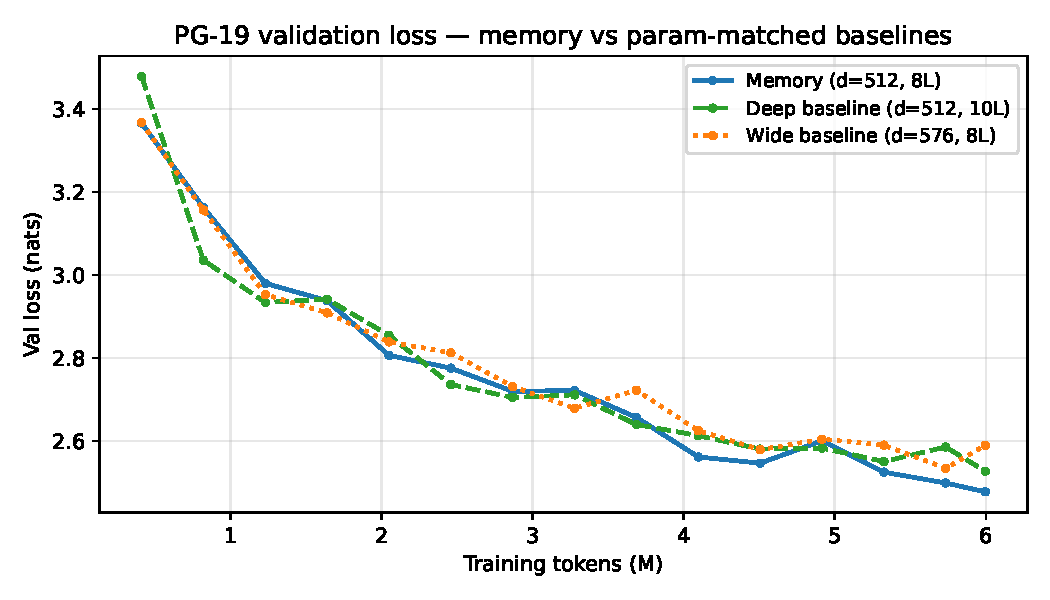
\includegraphics[width=0.85\textwidth]{figures/prose_training.pdf}
\caption{PG-19 val loss over training. Val estimated over 10 random batches per checkpoint (noisy).}
\label{fig:prose_training}
\end{figure}

Val estimates are noisy (10 random batches per checkpoint); the trend should be interpreted cautiously. All models are still improving at 6M tokens (Figure~\ref{fig:prose_training}).

\FloatBarrier
\subsubsection*{Long-context evaluation: Prose (18M)}
Per-segment loss at 1K intervals, averaged over 8 random 16K-token windows from PG-19 val (memory vs.\ wide baseline, no fine-tuning):

\begin{table}[h]
\centering
\caption{Per-segment PG-19 val loss at 16K context ($8\times$ training length).}
\begin{tabular}{lrrr}
\toprule
Segment & Memory & Wide & Gap \\
\midrule
0K--1K   & 2.554 & 2.538 & $-$0.017 \\
1K--2K   & 2.502 & 2.517 & $+$0.016 \\
2K--3K   & 2.555 & 2.584 & $+$0.029 \\
3K--4K   & 2.512 & 2.561 & $+$0.049 \\
4K--5K   & 2.496 & 2.519 & $+$0.023 \\
5K--6K   & 2.516 & 2.545 & $+$0.029 \\
6K--7K   & 2.441 & 2.444 & $+$0.003 \\
7K--8K   & 2.440 & 2.470 & $+$0.031 \\
8K--9K   & 2.408 & 2.436 & $+$0.028 \\
9K--10K  & 2.443 & 2.487 & $+$0.043 \\
10K--11K & 2.457 & 2.487 & $+$0.030 \\
11K--12K & 2.450 & 2.461 & $+$0.010 \\
12K--13K & 2.474 & 2.502 & $+$0.028 \\
13K--14K & 2.447 & 2.455 & $+$0.008 \\
14K--15K & 2.480 & 2.480 & $+$0.000 \\
15K--16K & 2.533 & 2.520 & $-$0.013 \\
\midrule
Overall  & 2.482 & 2.500 & $+$0.019 \\
\bottomrule
\end{tabular}
\end{table}

Memory wins on 13 of 16 segments. The gap is modest and noisy --- prose lacks the dense repeated-identifier structure that lets $W$ accumulate strong associations. At 64K ($32\times$ training length) the overall gap widens slightly to $+$0.028 (memory 2.484, wide 2.512). The effect is substantially larger on structured code, where identifier reuse gives $W$ much clearer associations to exploit (Section~\ref{sec:code}).

\FloatBarrier
\subsection{Code (Headline Result)}
\label{sec:code}

We train on Python files from codeparrot/codeparrot-clean (files $\geq$4096 chars), using a 512-vocab BPE tokenizer (${\sim}$16M tokens). Memory: 8-layer, 18.0M params; deep baseline: 10-layer, 17.2M params. Both trained identically, except the cosine LR horizon was set to ${\sim}$500K steps --- far beyond the 1465-step run --- so LR was near-peak throughout (caveat: results may differ under a tuned schedule).

\begin{table}[h]
\centering
\caption{Python code val loss (nats) during training, with PPL at the final checkpoint.}
\begin{tabular}{lrrrrr}
\toprule
Tokens & Memory & Deep & Gap & PPL (Mem / Deep) \\
\midrule
0.4M & 3.207 & 3.782 & $+$0.575 & --- \\
0.8M & 2.739 & 3.329 & $+$0.590 & --- \\
2.0M & 2.195 & 3.215 & $+$1.021 & --- \\
4.1M & 2.024 & 2.571 & $+$0.547 & --- \\
\midrule
6.0M & \textbf{1.848} & 2.787 & $+$0.939 & 6.35 / 16.24 \\
\bottomrule
\end{tabular}
\end{table}

The gap ($+$0.939 nats) is ${\sim}8\times$ larger than the prose gap against the deep baseline ($+$0.112 nats). Memory surpasses the baseline's final val loss by step 200 (${\sim}$800K tokens, 14\% of training; Figure~\ref{fig:code_training}).

\begin{figure}[h]
\centering
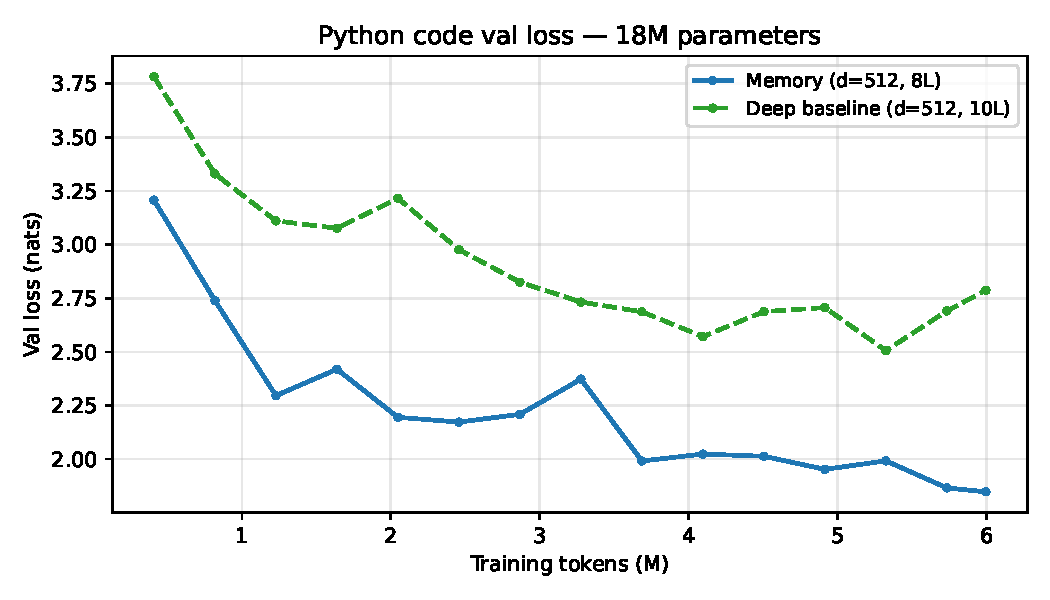
\includegraphics[width=0.85\textwidth]{figures/code_training_18M.pdf}
\caption{Python code val loss over training (18M models, 6M tokens). Memory leads throughout.}
\label{fig:code_training}
\end{figure}

\FloatBarrier
\subsubsection*{W ablation}
To confirm that $W$ itself (not just the additional parameters) drives the improvement, we compare two inference passes on the trained 18M code model: normal ($W$ updating each step) vs.\ frozen ($W$ reset to its pre-step value, so it never accumulates). Evaluated over 8 random 16K-token windows:

\begin{table}[h]
\centering
\caption{W ablation on 18M code model (8 windows $\times$ 16K tokens).}
\begin{tabular}{lrr}
\toprule
 & Val Loss & vs.\ updating \\
\midrule
$W$ updating (normal) & 1.940 & --- \\
$W$ frozen            & 2.877 & $+$0.938 \\
\bottomrule
\end{tabular}
\end{table}

Freezing $W$ costs 0.938 nats --- nearly equal to the full memory-vs-baseline gap of 0.939. The improvement comes from $W$, not from the extra parameters. Notably, the per-segment delta grows with context: $+$0.74 nats at 0--1K rising to $+$1.11 nats at 14--15K (Figure~\ref{fig:w_ablation}), confirming that $W$ accumulates associations over time rather than relying solely on immediate context.

\begin{figure}[h]
\centering

\includegraphics[width=0.85\textwidth]{eval_memory/eval_memory.png}
\caption{Per-segment loss for updating vs.\ frozen $W$ on the 18M code model (8 $\times$ 16K tokens). The gap widens with context as $W$ accumulates associations.}
\label{fig:w_ablation}
\end{figure}

\FloatBarrier
\subsubsection*{Long-context evaluation: Code (18M, codeparrot)}
We evaluate both 18M code models on 4 random 16K-token windows ($8\times$ training length) from the code val set, with no fine-tuning, measuring per-segment loss at 1K intervals (averaged over windows):

\begin{table}[h]
\centering
\begin{tabular}{lrrr}
\toprule
Segment & Memory & Deep & Gap \\
\midrule
0K--1K   & 2.203 & 2.650 & $+$0.447 \\
1K--2K   & 2.170 & 2.631 & $+$0.461 \\
2K--3K   & 2.011 & 2.632 & $+$0.622 \\
3K--4K   & 2.134 & 2.761 & $+$0.627 \\
4K--5K   & 2.068 & 2.631 & $+$0.562 \\
5K--6K   & 1.940 & 2.790 & $+$0.850 \\
6K--7K   & 1.960 & 2.891 & $+$0.931 \\
7K--8K   & 1.631 & 2.698 & $+$1.067 \\
8K--9K   & 1.834 & 2.719 & $+$0.885 \\
9K--10K  & 2.012 & 2.698 & $+$0.686 \\
10K--11K & 1.992 & 2.686 & $+$0.694 \\
11K--12K & 2.034 & 2.678 & $+$0.645 \\
12K--13K & 1.893 & 2.802 & $+$0.910 \\
13K--14K & 1.574 & 2.327 & $+$0.753 \\
14K--15K & 1.460 & 2.451 & $+$0.992 \\
15K--16K & 1.676 & 2.484 & $+$0.809 \\
\midrule
Overall  & 1.912 & 2.658 & $+$0.746 \\
\bottomrule
\end{tabular}
\end{table}

Memory wins every segment. The gap grows from $+$0.447 at 0--1K to $+$1.067 at 7--8K, peaks again at 14K--15K ($+$0.992), as $W$ accumulates file-level associations. Identifiers referenced late in a file were first defined early; by the time the usage site appears, $W$ has stored the (predecessor-of-definition, post-definition state) pair and retrieves it directly. The baseline must instead retain all bindings through its 16-dimensional recurrent state across thousands of intervening tokens.

\FloatBarrier
\subsection{Model Size Scaling: 18M $\to$ 100M}

We scale to 100M parameters on the same Python code dataset (512-vocab BPE, ${\sim}$16M tokens), training both models identically: $B{=}1$, $T{=}2048$, 8000 steps (16.4M tokens), constant LR $3{\times}10^{-4}$, $\alpha{=}0.05$. Val loss is measured on a single batch (20K tokens); readings have high variance but the trend is unambiguous.

\begin{table}[h]
\centering
\caption{100M training dynamics on Python code. Bold marks each model's best checkpoint.}
\begin{tabular}{lrrr}
\toprule
Tokens & Memory & Deep & Gap \\
\midrule
0.4M  & 3.353 & 3.984 & $+$0.631 \\
2.0M  & 2.215 & 2.898 & $+$0.683 \\
4.1M  & 2.159 & 2.866 & $+$0.707 \\
8.2M  & 1.993 & 2.273 & $+$0.280 \\
12.3M & 1.733 & 2.264 & $+$0.531 \\
14.7M & \textbf{1.661} & 2.182 & $+$0.521 \\
15.6M & 1.747 & \textbf{1.968} & $+$0.221 \\
\midrule
16.4M & 1.846 & 2.187 & $+$0.341 \\
\midrule
Best  & \textbf{1.661} & \textbf{1.968} & $+$0.307 \\
\bottomrule
\end{tabular}
\end{table}

Memory leads at every checkpoint; the gap peaks at 4M tokens ($+$0.707) before closing as the stronger baseline catches up (Figure~\ref{fig:code_training_100M}). The 18M memory model outperforms the 100M deep baseline at every checkpoint in the 100M model's training run --- including its best checkpoint (1.968 vs.\ 1.848) --- at $5.6\times$ fewer parameters and $2.7\times$ fewer training tokens.

\begin{figure}[h]
\centering
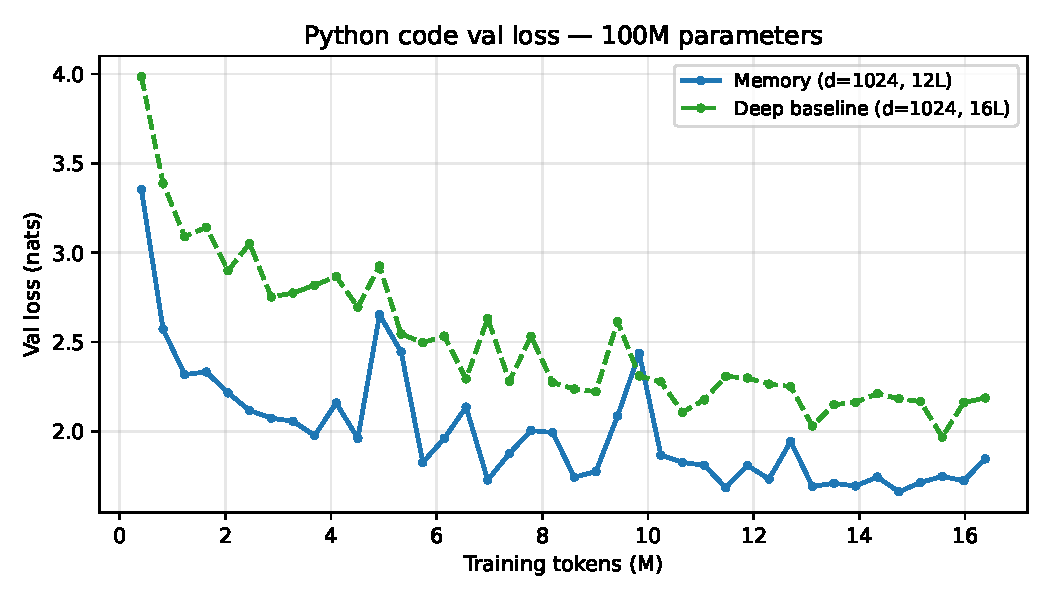
\includegraphics[width=0.85\textwidth]{figures/code_training_100M.pdf}
\caption{Python code val loss over training (100M models, 16.4M tokens). Memory leads at every checkpoint.}
\label{fig:code_training_100M}
\end{figure}

The narrowed gap at 100M ($+$0.307 vs.\ $+$0.939 at 18M) reflects a stronger baseline: best val 1.968 vs.\ 2.787, leaving less headroom.

\FloatBarrier
\subsubsection*{Long-context evaluation: Code (100M, codeparrot)}
Per-segment loss at 1K intervals, averaged over 8 random 16K-token windows (no fine-tuning):

\begin{table}[h]
\centering
\caption{Per-segment val loss at 16K context, 100M models (8 windows, 1K segments).}
\begin{tabular}{lrrr}
\toprule
Segment & Memory & Deep & Gap \\
\midrule
0K--1K   & 1.902 & 2.230 & $+$0.328 \\
1K--2K   & 1.660 & 2.112 & $+$0.452 \\
2K--3K   & 1.572 & 2.066 & $+$0.494 \\
3K--4K   & 1.844 & 2.212 & $+$0.368 \\
4K--5K   & 1.827 & 2.138 & $+$0.311 \\
5K--6K   & 1.805 & 2.223 & $+$0.418 \\
6K--7K   & 1.768 & 2.217 & $+$0.449 \\
7K--8K   & 1.580 & 2.153 & $+$0.572 \\
8K--9K   & 1.744 & 2.144 & $+$0.400 \\
9K--10K  & 1.759 & 2.133 & $+$0.374 \\
10K--11K & 1.732 & 2.163 & $+$0.430 \\
11K--12K & 1.797 & 2.171 & $+$0.374 \\
12K--13K & 1.749 & 2.205 & $+$0.456 \\
13K--14K & 1.405 & 1.821 & $+$0.416 \\
14K--15K & 1.302 & 1.791 & $+$0.489 \\
15K--16K & 1.512 & 1.961 & $+$0.449 \\
\midrule
Overall  & \textbf{1.685} & 2.109 & $+$0.424 \\
\bottomrule
\end{tabular}
\end{table}

Memory wins every segment. Unlike the 18M model where the gap peaked at 7--8K, the 100M memory model continues improving to 14--15K tokens, with the larger $W$ ($1024{\times}1024$) accumulating associations across the full window. Figure~\ref{fig:long_context_100M} shows the full per-segment profile.

\begin{figure}[h]
\centering
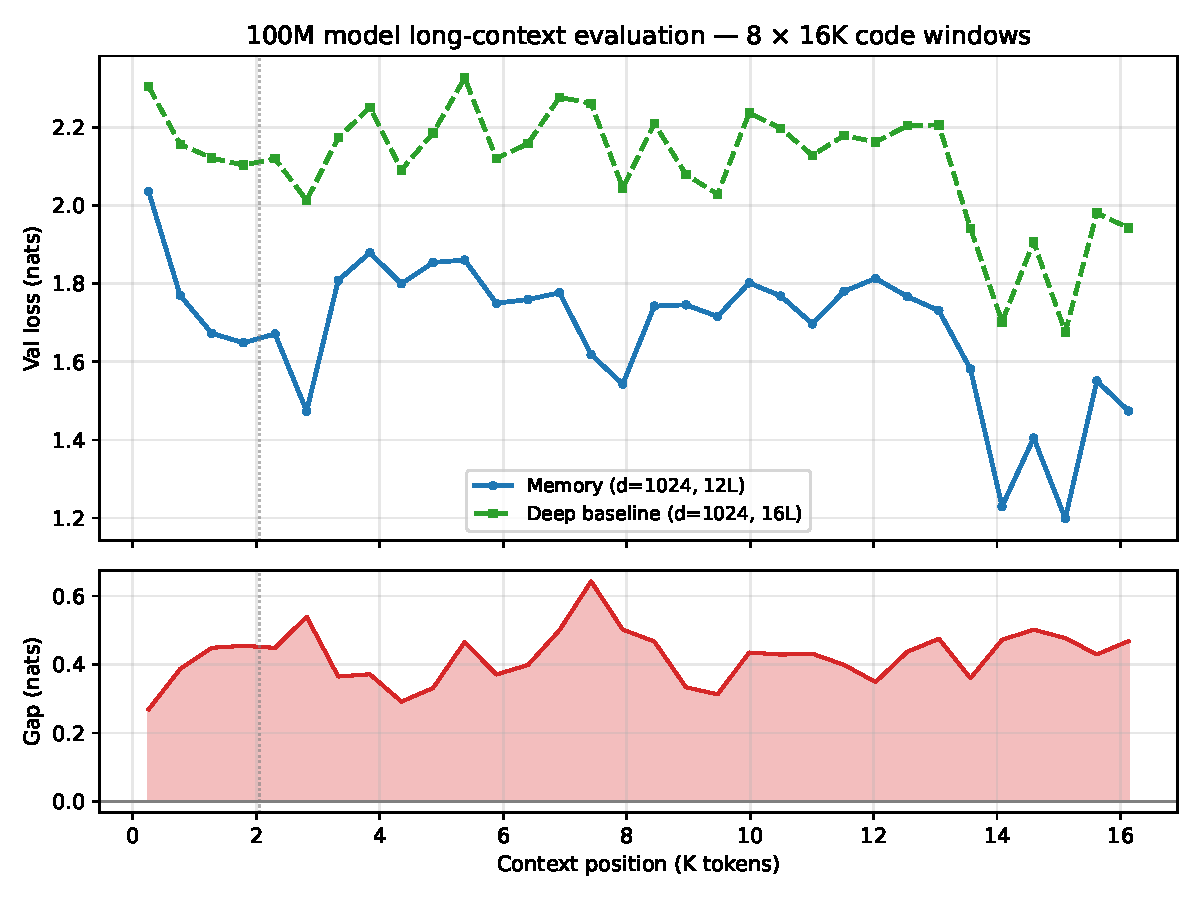
\includegraphics[width=0.9\textwidth]{figures/long_context_100M.pdf}
\caption{100M model per-segment val loss and gap over 16K context. Vertical dotted line marks training length (2K tokens).}
\label{fig:long_context_100M}
\end{figure}

\FloatBarrier
\subsubsection*{Learned decay ($\gamma$)}
At 18M, all 8 layers converge to $\gamma \approx 0.990$--$0.993$ (windows 97--144 steps) with little specialization. At 100M, layers 1--5 develop long-range associations ($\gamma \approx 0.996$--$0.997$, windows 250--355 steps) while layer 0 and layers 6--11 stay short-range ($\gamma \approx 0.979$--$0.992$, windows 48--125 steps). Layer specialization only emerges at the larger scale (Figure~\ref{fig:decay_gamma}).

\begin{figure}[h]
\centering
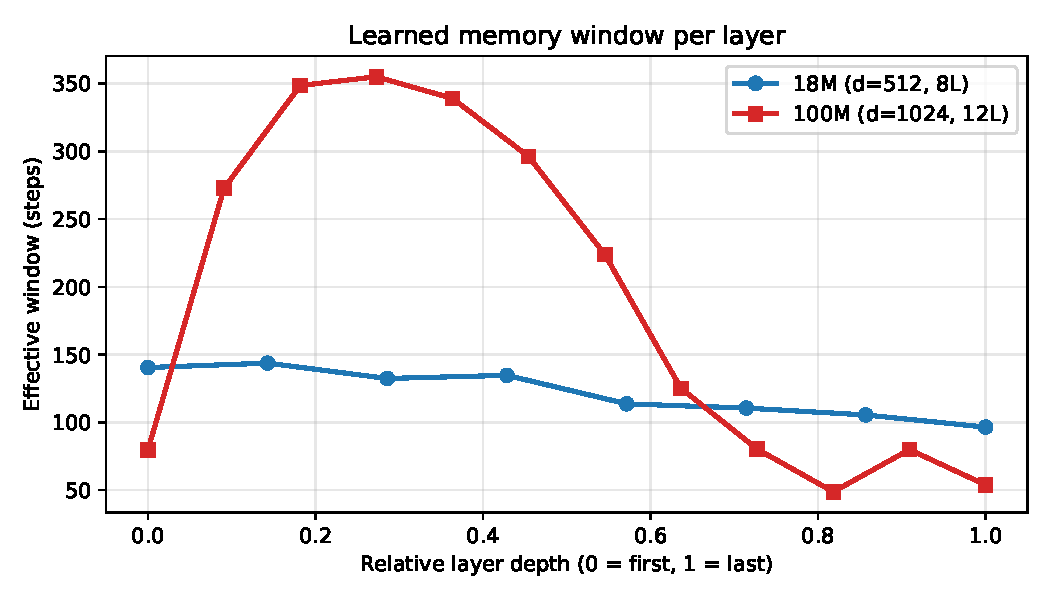
\includegraphics[width=0.9\textwidth]{figures/decay_gamma.pdf}
\caption{Learned effective memory window per layer ($= 1/(1-\gamma)$) for the 18M and 100M code memory models.}
\label{fig:decay_gamma}
\end{figure}

\FloatBarrier
\subsection{Dataset Breadth: Multilingual Code (The Stack)}

We train 100M models on The Stack \citep{kocetkov2022stack}: eight languages (Python, JavaScript, TypeScript, Java, C, C\texttt{++}, Rust, Go), files ${\geq}32{,}000$ chars, ${\sim}$14.5M training tokens. We increase the BPE vocabulary to 1024 (from 512 used in previous experiments): a larger vocabulary provides more distinct token identities as write keys, reducing key collision in $W$ and giving the associative matrix more signal to exploit. Memory: 97.5M (11L), deep baseline: 101.1M (15L), $\alpha{=}0.04$. Both models are undertrained at 8.2M tokens; best-vs-best gap is $+$0.263 nats (1.621 vs.\ 1.884; Figure~\ref{fig:stack_training}).

\begin{table}[h]
\centering
\caption{The Stack 100M training dynamics. Bold marks each model's best checkpoint.}
\begin{tabular}{lrrr}
\toprule
Tokens & Memory & Deep & Gap \\
\midrule
0.4M & 5.044 & 5.354 & $+$0.310 \\
0.8M & 3.251 & 4.454 & $+$1.203 \\
2.1M & 2.237 & 3.102 & $+$0.865 \\
4.1M & 1.919 & 2.370 & $+$0.451 \\
6.1M & 1.678 & 2.576 & $+$0.898 \\
\midrule
8.2M & 1.923 & 2.049 & $+$0.126 \\
\midrule
Best & \textbf{1.621} & \textbf{1.884} & $+$0.263 \\
\bottomrule
\end{tabular}
\end{table}

\begin{figure}[h]
\centering
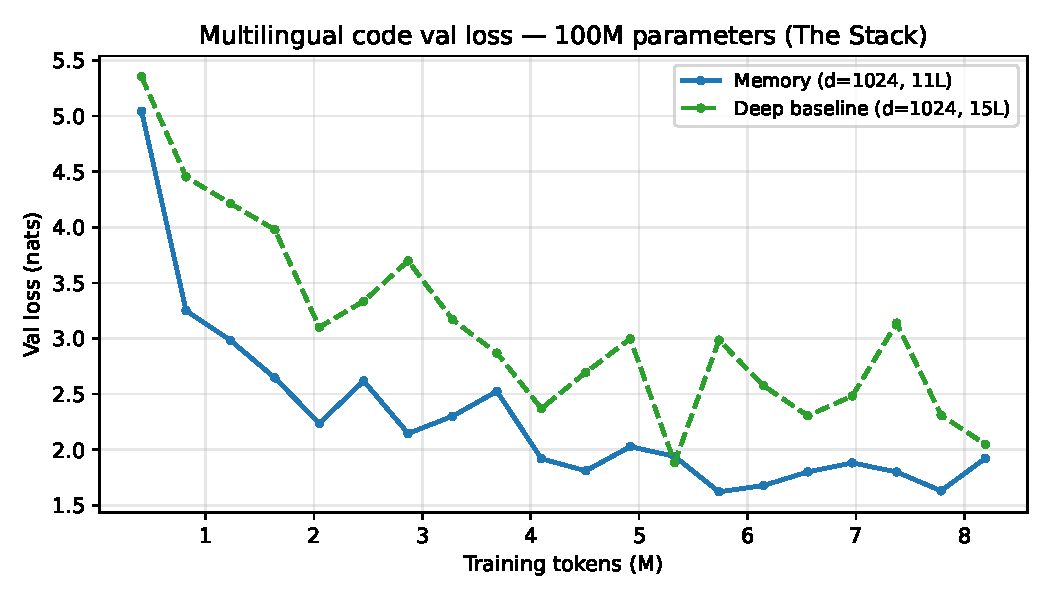
\includegraphics[width=0.85\textwidth]{figures/stack_training_100M.pdf}
\caption{Multilingual code (The Stack) val loss over training, 100M models.}
\label{fig:stack_training}
\end{figure}

\FloatBarrier
\subsubsection*{Long-context evaluation: Code (100M, The Stack)}
Per-segment loss at 1K intervals, averaged over 8 random 16K-token windows (no fine-tuning):

\begin{table}[h]
\centering
\caption{Per-segment val loss at 16K context, Stack 100M (8 windows, 1K segments).}
\begin{tabular}{lrrr}
\toprule
Segment & Memory & Deep & Gap \\
\midrule
0K--1K   & 1.452 & 2.097 & $+$0.645 \\
1K--2K   & 1.235 & 2.067 & $+$0.831 \\
2K--3K   & 1.295 & 2.067 & $+$0.772 \\
3K--4K   & 1.344 & 2.244 & $+$0.901 \\
4K--5K   & 1.194 & 2.061 & $+$0.867 \\
5K--6K   & 1.332 & 2.199 & $+$0.867 \\
6K--7K   & 1.622 & 2.435 & $+$0.813 \\
7K--8K   & 1.618 & 2.437 & $+$0.819 \\
8K--9K   & 1.487 & 2.152 & $+$0.665 \\
9K--10K  & 1.464 & 2.027 & $+$0.563 \\
10K--11K & 1.397 & 1.854 & $+$0.457 \\
11K--12K & 1.575 & 1.973 & $+$0.398 \\
12K--13K & 1.534 & 1.969 & $+$0.435 \\
13K--14K & 1.602 & 2.149 & $+$0.548 \\
14K--15K & 1.624 & 1.870 & $+$0.246 \\
15K--16K & 1.477 & 1.873 & $+$0.397 \\
\midrule
Overall  & \textbf{1.453} & 2.092 & $+$0.639 \\
\bottomrule
\end{tabular}
\end{table}

Memory wins all 16 segments. The overall gap ($+$0.639) exceeds the Python 100M result ($+$0.424), consistent with the richer vocabulary and longer files providing denser associations for $W$. On the two densest individual windows, the deep baseline's overall loss reaches ${\sim}3.05$ nats while memory stays at ${\sim}1.67$ nats (Figure~\ref{fig:long_context_stack}; these per-window averages are not visible in the per-segment table above, which averages across all 8 windows).

\begin{figure}[h]
\centering
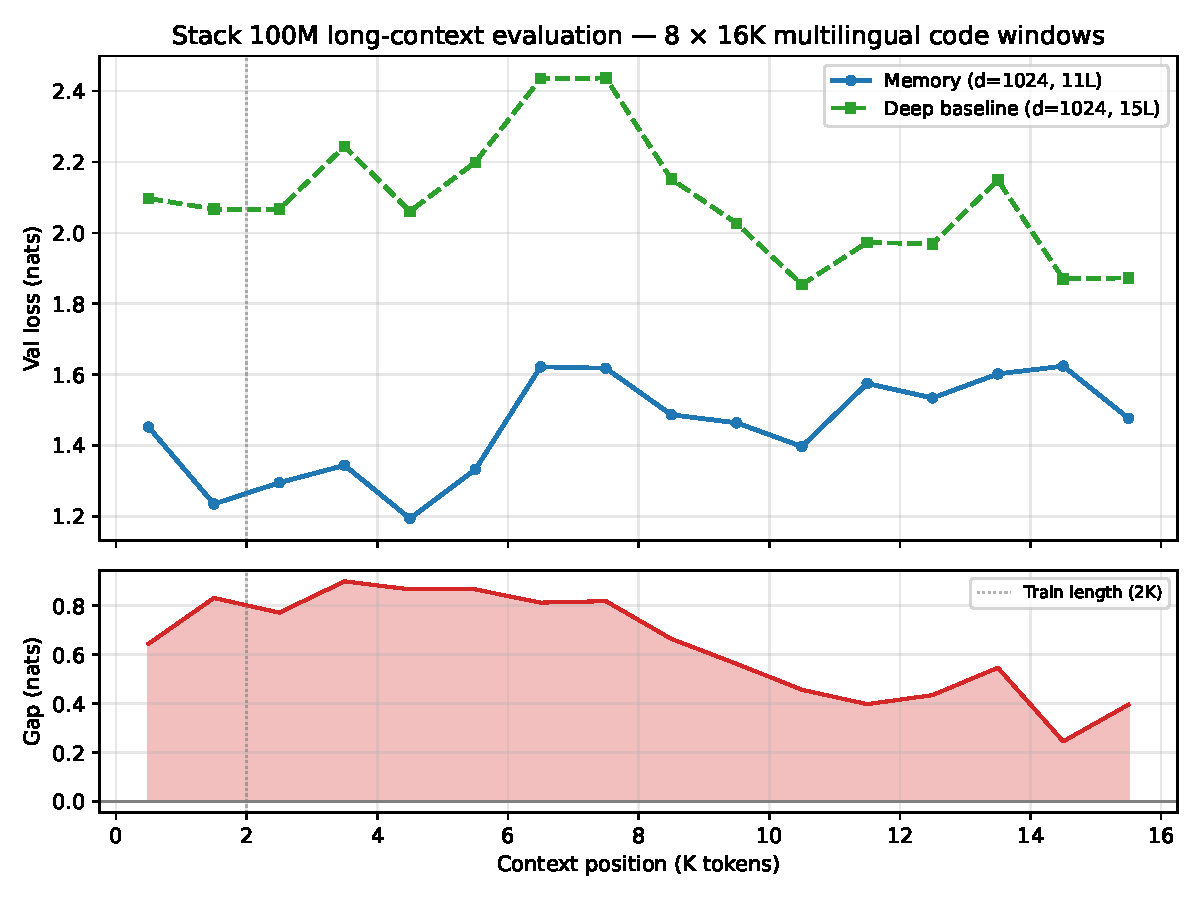
\includegraphics[width=0.9\textwidth]{figures/long_context_stack.pdf}
\caption{Stack 100M per-segment val loss and gap over 16K context. Vertical dotted line marks training length (2K tokens).}
\label{fig:long_context_stack}
\end{figure}

\clearpage
\section{Related Work}

\paragraph{Fast weights.}
The closest prior work is Ba et al.~\citep{ba2016using}, who augment an RNN with a fast weight matrix updated by outer products of hidden states: $W_t = \lambda W_{t-1} + \eta\, h_t h_t^\top$, with retrieval via iterative inner-loop steps. Schmidhuber~\citep{schmidhuber1992learning} proposed fast-weight memories earlier in a metalearning context. Our $W$ follows the same outer-product-plus-decay principle but makes three changes: (1) decoupling write and read keys via learned projections --- necessary for correct retrieval after Mamba state resets, as shown in Section~\ref{sec:recall}; (2) using a fixed injection scale $\alpha$ rather than a learned gate, preventing memory noise from destabilizing early training; and (3) admitting a parallel scan formulation (Section~\ref{sec:method}) that makes training as efficient as Mamba itself, unlike Ba et al.'s sequential inner-loop retrieval.

\paragraph{External and associative memory.}
Neural Turing Machines \citep{graves2014neural} and Differentiable Neural Computers \citep{graves2016hybrid} maintain an external memory bank with learned content-based read and write heads. Our $W$ is simpler: a single $d \times d$ matrix updated by a fixed rule, trading capacity for constant per-step cost. Modern Hopfield Networks \citep{ramsauer2021hopfield} show that softmax attention computes energy-minimizing retrievals in a Hopfield associative memory; our $W$ implements an unnormalized causal variant with strict causal masking and separate write/read projections. These mechanisms are specific to SSMs: in a Transformer, the KV cache retains all past tokens within the context window, leaving no gap for an additional memory matrix.

\paragraph{Memory in SSMs.}
Test-Time Training \citep[TTT;][]{sun2024learning} is an RNN-like model whose hidden state is a weight matrix updated by gradient descent on a self-supervised loss at each step. Titans \citep{behrouz2024titans} combine a similar gradient-based neural memory module with sliding-window attention in a hybrid transformer. MesaNet \citep{von2025mesanet} pushes this further by solving the in-context optimization to near-optimality using conjugate gradient steps; while it supports chunkwise parallelization within chunks, the inter-chunk CG iterations are inherently sequential and do not batch efficiently across long sequences. All three learn their update rule end-to-end through an inner-loop optimization, incurring significant per-step overhead. Our $W$ uses a fixed outer-product rule with no inner loop: $O(d^2)$ per step, purely feedforward, and trivially batchable --- at the cost of a less expressive update.

\paragraph{Linear recurrences and the delta rule.}
RetNet \citep{sun2023retentive}, RWKV \citep{peng2023rwkv}, and Gated Linear Attention \citep{yang2023gated} reformulate causal attention as a linear recurrence, achieving $O(1)$ state per step. Mamba-2 \citep{dao2024mamba2} establishes a structured state-space duality (SSD) showing that Mamba's selective scan is equivalent to a form of linear attention. Schlag et al.~\citep{schlag2021linear} make the connection explicit: linear attention is equivalent to a fast-weight programmer using Hebbian outer-product writes. DeltaNet \citep{yang2024deltanet} replaces the outer product with the error-corrective delta rule: $W_t \leftarrow W_{t-1} + \beta_t(v_t - W_{t-1}k_t)k_t^\top$, actively removing stale associations before writing new ones, which reduces interference more directly than exponential decay. LUCID \citep{duvvuri2026lucid} derives causal attention as the delta rule in an RKHS and applies a key--key preconditioner to decorrelate queries, improving long-context recall in transformers --- but the method is applied to transformers and remains $O(T^2)$ in sequence length; the preconditioner helps attention \emph{forget} stale associations more cleanly, not avoid the quadratic cost. Our $W$ is $O(Td^2)$: linear in sequence length, at the cost of bounded associative capacity.

\section{Conclusion}

SSMs have a lossy state bottleneck; code is associative recall. A Hebbian $W$ fills the gap: drop-in (32 lines, no training changes), $O(Td^2)$ in sequence length, and compute-efficient --- the 18M memory model outperforms the 100M deep baseline at $5.6\times$ fewer parameters. The advantage persists to 16K tokens ($8\times$ training length) across all settings, while quadratic alternatives become intractable at exactly the contexts where associative recall matters most.

At 18M parameters, the memory model reaches 1.848 nats on Python code versus 2.787 for a parameter-matched baseline ($+$0.939 nats), surpassing the baseline's final validation loss after only 800K tokens and outperforming the 100M baseline throughout its entire training run. At 100M parameters the best-checkpoint gap is $+$0.307 nats on Python and $+$0.639 nats at 16K tokens on multilingual code (The Stack) --- the largest gap we observe. On prose the effect is smaller but consistent (2.477 vs.\ 2.527), suggesting the mechanism is broadly useful and especially powerful when data is highly associative.

\subsection*{Scaling Properties}
In theory, several factors should compound favourably as scale increases:
\begin{itemize}
  \item \textbf{Associative capacity.} $W$ supports ${\sim}d$ approximately orthogonal associations per layer. At larger $d$, capacity grows and inter-association interference decreases, allowing richer retrieval without architectural changes.
  \item \textbf{Longer context, more signal.} Every additional token is a write opportunity. At production context lengths (hundreds of thousands of tokens), $W$ has orders of magnitude more associations to exploit than in our experiments.
  \item \textbf{Domain density.} Code, mathematics, and formal logic are dense in reusable symbol patterns --- variable names, function signatures, theorem components. The denser the associative structure, the more $W$ has to exploit; the Stack gap ($+$0.639) exceeding the Python gap ($+$0.424) is consistent with this, and harder domains (multi-file repositories, mathematical proofs) should widen it further.
\end{itemize}
We conjecture that $W$'s relative benefit is governed by task difficulty: as the baseline grows stronger it handles more of the problem on its own, shrinking the gap (as seen at 100M vs.\ 18M). But difficulty grows faster than baseline capability --- harder corpora, longer contexts, denser symbol reuse --- and $W$ fills exactly the associative gap the baseline leaves. The implication is that the gap should widen again on problems that are genuinely hard for the recurrent state to handle alone.

\subsection*{Limitations}
$W$'s two projection matrices add roughly 25\% to parameter count per layer. The real constraints are associative capacity (${\sim}d$ orthogonal associations per layer) and the single scalar decay per layer, which cannot differentiate retention by content or recency beyond a fixed exponential. The prose experiments used a cosine LR schedule set to complete at 6M tokens before it was clear models were undertrained; the reported gaps are conservative lower bounds. We have only evaluated on Mamba; transfer to other SSMs is straightforward but untested.

All experiments were run on a single MacBook Pro (Apple M-series, 24\,GB unified memory) using PyTorch MPS. This imposes practical constraints: bf16 is unsupported for some operations on MPS, batch sizes are small, and 100M-parameter runs take days. Results have not been reproduced on GPU hardware. This paper was written with substantial assistance from a large language model (Claude); all experimental results, code, and final editorial judgements are the author's own.

\subsection*{Future Directions}
\begin{itemize}
  \item \textbf{Training}: longer sequences (gradient signal for longer-range associations), harder datasets (multi-document QA, multi-file repositories).
  \item \textbf{Memory design}: a secondary $W$ with slower decay to capture a different timescale; learnable or input-dependent $\alpha$; per-layer decay specialization.
  \item \textbf{Efficiency}: bf16/low-precision storage and update of $W$ without capacity loss.
  \item \textbf{Continual learning}: $W$ already implements online associative updates without gradient descent; no replay buffer or task boundary needed.
  \item \textbf{Other modalities}: Vision Mamba processes patches in a fixed scan order; $W$ could bind patch identities on first encounter rather than relying on the recurrent state to carry them. Video is similarly associative (objects and scenes reappearing across cuts).
\end{itemize}

\begin{thebibliography}{10}

\bibitem{elhage2022superposition}
Nelson Elhage, Tristan Hume, Catherine Olsson, Nicholas Schiefer, Tom Henighan, Shauna Kravec, Zac Hatfield-Dodds, Robert Lasenby, Dawn Drain, Carol Chen, Roger Grosse, Sam McCandlish, Jared Kaplan, Dario Amodei, Martin Wattenberg, and Christopher Olah.
\newblock Toy models of superposition.
\newblock \emph{Transformer Circuits Thread}, 2022.

\bibitem[Ba et~al.(2016)]{ba2016using}
Jimmy Ba, Geoffrey Hinton, Volodymyr Mnih, Joel~Z. Leibo, and Catalin Ionescu.
\newblock Using fast weights to attend to the recent past.
\newblock In \emph{Advances in Neural Information Processing Systems}, 2016.

\bibitem{behrouz2024titans}
Ali Behrouz, Peilin Zhong, and Vahab Mirrokni.
\newblock Titans: Learning to memorize at test time.
\newblock \emph{arXiv preprint arXiv:2501.00663}, 2025.

\bibitem{duvvuri2026lucid}
Sai Surya Duvvuri, Nirmal Patel, Nilesh Gupta, and Inderjit~S. Dhillon.
\newblock {LUCID}: Attention with preconditioned representations.
\newblock \emph{arXiv preprint arXiv:2602.10410}, 2026.

\bibitem{graves2014neural}
Alex Graves, Greg Wayne, and Ivo Danihelka.
\newblock Neural turing machines.
\newblock \emph{arXiv preprint arXiv:1410.5401}, 2014.

\bibitem{graves2016hybrid}
Alex Graves, Greg Wayne, Malcolm Reynolds, Tim Harley, Ivo Danihelka,
  Agnieszka Grabska-Barwi{\'n}ska, Sergio~G{\'o}mez Colmenarejo, Edward
  Grefenstette, Tiago Ramalho, John Agapiou, et~al.
\newblock Hybrid computing using a neural network with dynamic external memory.
\newblock \emph{Nature}, 538(7626):471--476, 2016.

\bibitem{gu2023mamba}
Albert Gu and Tri Dao.
\newblock Mamba: Linear-time sequence modeling with selective state spaces.
\newblock \emph{arXiv preprint arXiv:2312.00752}, 2023.

\bibitem{dao2024mamba2}
Tri Dao and Albert Gu.
\newblock Transformers are {SSMs}: Generalized models and efficient algorithms through structured state space duality.
\newblock \emph{arXiv preprint arXiv:2405.21060}, 2024.

\bibitem{peng2023rwkv}
Bo~Peng, Eric Alcaide, Quentin Anthony, Alon Albalak, Samuel Arcadinho,
  Huanqi Cao, Xin Cheng, Michael Chung, Matteo Grella, Kranthi~Kiran~GV,
  et~al.
\newblock {RWKV}: Reinventing {RNN}s for the transformer era.
\newblock In \emph{Findings of EMNLP}, 2023.

\bibitem{ramsauer2021hopfield}
Hubert Ramsauer, Bernhard Sch{\"a}fl, Johannes Lehner, Philipp Seidl, Michael
  Widrich, Thomas Adler, Lukas Gruber, Markus Holzleitner, Milena Pavlovic,
  Geir~Kjetil Stormo, et~al.
\newblock Hopfield networks is all you need.
\newblock In \emph{International Conference on Learning Representations}, 2021.

\bibitem{von2025mesanet}
Johannes von~Oswald, Nino Scherrer, Seijin Kobayashi, Luca Versari, Songlin Yang,
  Maximilian Schlegel, Kaitlin Maile, Yanick Schimpf, Oliver Sieberling,
  Alexander Meulemans, et~al.
\newblock {MesaNet}: Sequence modeling by locally optimal test-time training.
\newblock \emph{arXiv preprint arXiv:2506.05233}, 2025.

\bibitem[Schmidhuber(1992)]{schmidhuber1992learning}
J{\"u}rgen Schmidhuber.
\newblock Learning to control fast-weight memories: An alternative to recurrent
  nets.
\newblock \emph{Neural Computation}, 4(1):131--139, 1992.

\bibitem{sun2023retentive}
Yutao Sun, Li~Dong, Shaohan Huang, Shuming Ma, Yuqing Xia, Jilong Xue,
  Jianyong Wang, and Furu Wei.
\newblock Retentive network: A successor to transformer for large language
  models.
\newblock \emph{arXiv preprint arXiv:2307.08621}, 2023.

\bibitem{sun2024learning}
Yu~Sun, Xinhao Li, Karan Dalal, Jiarui Xu, Arjun Aghajanyan, Gregory~W.
  Wornell, Xinlei Chen, and Mike Lewis.
\newblock Learning to (learn at test time): {RNN}s with expressive hidden
  states.
\newblock \emph{arXiv preprint arXiv:2407.04620}, 2024.

\bibitem{yang2023gated}
Songlin Yang, Bailin Wang, Yikang Shen, Rameswar Panda, and Yoon Kim.
\newblock Gated linear attention transformers with hardware-efficient training.
\newblock \emph{arXiv preprint arXiv:2312.06635}, 2023.

\bibitem{kocetkov2022stack}
Denis Kocetkov, Raymond Li, Loubna Ben~Allal, Jia Li, Chenghao Mou,
  Carlos~Mu{\~n}oz Ferrandis, Yacine Jernite, Margaret Mitchell, Sean Hughes,
  Thomas Wolf, et~al.
\newblock The stack: 3 {TB} of permissively licensed source code.
\newblock \emph{arXiv preprint arXiv:2211.15533}, 2022.

\bibitem{yang2024deltanet}
Songlin Yang, Bailin Wang, Yu~Zhang, Yikang Shen, and Yoon Kim.
\newblock Parallelizing linear transformers with the delta rule over sequence length.
\newblock In \emph{Advances in Neural Information Processing Systems}, 2024.

\bibitem[Schlag et~al.(2021)]{schlag2021linear}
Imanol Schlag, Kazuki Irie, and J{\"u}rgen Schmidhuber.
\newblock Linear transformers are secretly fast weight programmers.
\newblock In \emph{International Conference on Machine Learning}, 2021.

\end{thebibliography}

\end{document}
